\subsection{Animation}

Für einer lebendige Szene in einem Spiel reicht es nicht aus nur statische Models zu verschieben und zu drehen. Wenn man zum Beispiel ein Pferdmodel im Spiel einbindet und es nur nach vorne bewegt, wenn es laufen soll, so wirkt das Pferd nicht lebendig und es sähe so aus, als würde man eine Statue verschieben. Man muss in diesem Falle also ein Modell animieren.

Die FM3D-Engine verwendet eine Animationsart namens \textit{Skeletal-Animation}. Hierbei bekommt jedes animierte Mesh ein Skelett zugewiesen, wobei sich mehrere verschiedene Meshes das gleiche Skelett teilen können. Zum Beispiel könnte es in einem Spiel ein Mesh für einen Ritter und eines für einen Bauern geben. Diese sehen unterschiedlich aus, aber beide könnten das gleiche Skelett und somit die gleichen Animationen haben.

Ein Skelett besteht aus mehreren Knochen, die jeweils an weiteren Knochen "`hängen"'. Wenn sich ein Knochen bewegt, bewegt er alle an ihm hängende Knochen und die wiederum alle an ihm hängenden. 
Dies hat den Vorteil, dass, wenn sich der Knochen des linken Armes bewegt, sich auch gleichzeitig alle Fingerknochen bewegen würden. Jeder Knochen besitzt unabhängig von den anderen eine Ausgangsposition und eine ID.
Die ID wird verwendet, um herauszufinden, welcher Knochen sich auf welchen Vertex auswirkt und welche Knochen nicht verwendet werden. Jeder Vertex kann von bis zu vier Knochen transformiert werden. Dazu besitzt jeder Vertex vier Knochen-IDs und vier Floats, die angeben, wie stark sich ein Knochen auf den Vertex auswirkt (Siehe \cref{table:VertexAufbau}). Diese Daten werden in einem externen Programm beim Erstellen des Meshes festgelegt. Dieser Vorgang wird \textit{Weight Painting} genannt, da die Zuweisung durch eine Art Malen in den Modellierungsprogrammen geschieht. Ein Beispiel aus dem Programm \textit{Blender} ist in \cref{Img:Skeleton} zu sehen.

Eine Animation besitzt zu verschiedenen Zeitpunkten eine Position, Rotation und Skalierung für einen Knochen genannt \textit{Keyframe}. Dabei ist es nicht nötig, dass alle Knochen die gleiche Anzahl an Keyframes haben oder einen Keyframe an der gleichen Zeitposition existiert. keine Position, Rotation und Skalierung auf einmal beinhalten, sondern nur eins oder zwei davon. Um den Zustand aller Knochen zu einem bestimmten Zeitpunkt herauszufinden, beginnt man am obersten Knochen der Hierarchie und arbeitet sich dann schrittweise nach unten, da die unteren Knochen von den oberen abhängig sind. 
Falls der Zustand zu diesem Zeitpunkt nicht zufällig durch die Keyframes genau definiert ist, muss zwischen den zwei am nächsten liegenden Keyframes interpoliert werden.

Für die Position und Skalierung kann zwischen den Keyframes linear interpoliert werden:

$t_{0} \leq t \leq t_{1}$ \qquad $t_{0} < t_{1}$ \qquad Keyframes: $\overrightarrow{P_{0}}, \overrightarrow{P_{1}}$

$f = \dfrac{t - t_{0}}{t_{1} - t_{0}}$

$\overrightarrow{P} = ((\overrightarrow{P_{0}} \cdot (1 - f)) + (\overrightarrow{P_{1}} \cdot f)$

Für die Rotation muss \ac{SLERP} \cite{WikiSlerp} angewendet werden, dadurch bleibt die Kreisgeschwindigkeit über die Zeit konstant. Die Berechnung erfolgt für zwei Quaternionen, die eine Rotation repräsentieren.
\todo[inline]{was sind Quaternionen}
$t_{0} \leq t \leq t_{1}$ \qquad $t_{0} < t_{1}$ \qquad Keyframes: $Q_{0}, Q_{1}$

$f = \dfrac{t - t_{0}}{t_{1} - t_{0}}$

$\phi = Q_{0} \cdot Q_{1}$

$\theta = \arccos(\phi) \cdot f$

$Q_{2} = Q_{1} - Q_{0} \cdot \phi$

$Q = Q_{0} \cdot \cos(\theta) + Q_{2} \cdot \sin(\theta)$

\begin{figure}
	\centering
	\begin{minipage}{0.49\textwidth}
		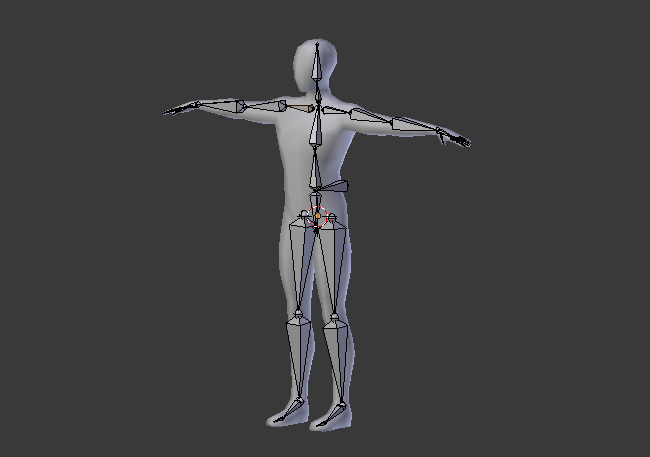
\includegraphics[width=\textwidth]{02theorie/skeleton.jpg}
	\end{minipage}
	\hfill
	\begin{minipage}{0.49\textwidth}
		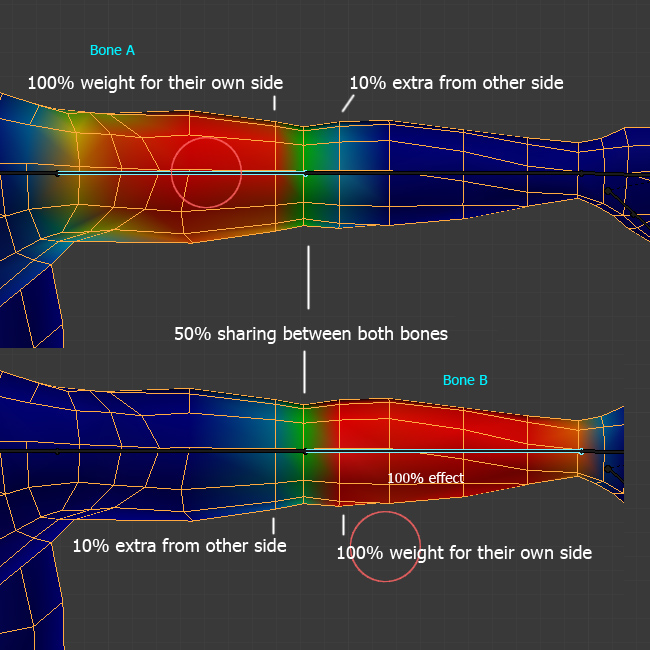
\includegraphics[width=\textwidth]{02theorie/weightpainting.jpg}
	\end{minipage}

	
	Links: Skelett in Blender, Rechts: Weight painting eines Arms in Blender 
	
	Quelle: https://cgi.tutsplus.com/tutorials/building-a-basic-low-poly-character-rig-in-blender--cg-16955
	\caption{Blender Skelett}\label{Img:Skeleton}
\end{figure}